\thesolution{Elimina Tutti}
Ipotizzando che l'elemento da eliminare sia 0, il metodo \cod{EliminaTutti()} modifica il vettore degli elementi come mostrato in \figurename~\ref{fig:EliminaTutti}.

\begin{figure}
  \center
	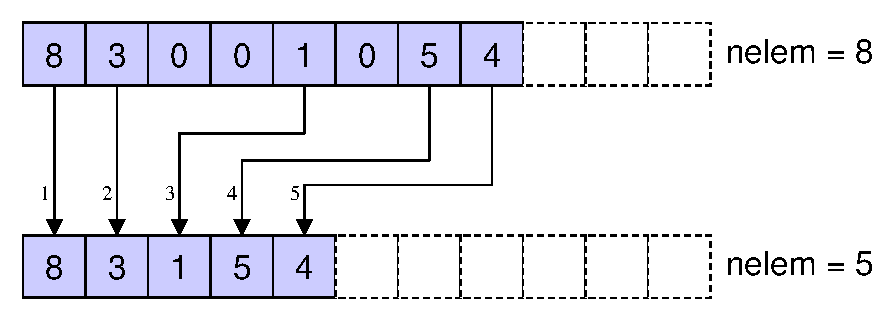
\includegraphics[width=.75\textwidth]{Esercizi/EliminaTutti/EliminaTutti.eps}
	\caption{Eliminazione degli elementi con valore 0 dal vettore}
	\label{fig:EliminaTutti}
\end{figure}

Per ottenere l'effetto desiderato � sufficiente scandire in sequenza gli elementi del vettore originario (in alto nella figura). Ad ogni passo, se l'elemento puntato � diverso dall'elemento da eliminare, lo si ricopia nel vettore in basso; in caso contrario non si effettua alcuna operazione e si passa ad analizzare l'elemento successivo. Alla fine della scansione il vettore in basso risulter� composto dai soli elementi del vettore originario diversi da quello da eliminare.

\`{E} facile convincersi del fatto che, per realizzare l'operazione appena descritta, non sia necessario utilizzare due distinti vettori, ma tutto il procedimento pu� essere svolto su un unico vettore. La copia di un elemento diviene in questo caso uno spostamento nell'ambito dello stesso vettore, senza che la sovrascrittura della locazione di destinazione rappresenti un problema. Allo scopo � sufficiente utilizzare due indici \cod{i} e \cod{j}:
\begin{itemize}
\item{\cod{i}} va da 0 a $\cod{nelem}-1$, scandendo in sequenza tutti gli elementi del vettore originario;
\item{\cod{j}} avanza ogni qual volta un elemento viene ``ricopiato'', e pertanto rappresenta il riempimento corrente del vettore ``ripulito''.
\end{itemize}

Di seguito si riporta il codice del metodo \cod{EliminaTutti()}.

\bigskip
\inputprogram{Esercizi/EliminaTutti/EliminaTutti.cpp}
\bigskip